\documentclass{phyasgn}
\phyasgn{
  stuname = 姚昊廷,           % 设置学生姓名
  stunum = 22322091,      % 设置学号
  setasgnnum = 1,           % 设置课程次数
  classname = 数学物理方法,     % 设置课程名称
}

\usepackage{listings}
\usepackage{tikz}
\usepackage{amssymb}
\usepackage{t-angles}
\usepackage{amssymb}
\usepackage{tikz}
\usepackage{mathrsfs}
\usepackage{pifont}
\usepackage{subfigure}
\usepackage{caption}
%\usepackage{autobreak} 
%\usepackage{fixdif} 
\usetikzlibrary{quotes,angles}
\usetikzlibrary{calc}
\usetikzlibrary{decorations.pathreplacing}
\lstset{numbers=left,basicstyle=\ttfamily,columns=flexible}
\makeatletter
\newcommand{\rmnum}[1]{\romannumeral #1}
\newcommand{\Rmnum}[1]{\expandafter\@slowromancap\romannumeral #1@}
\renewcommand{\i}{\mathrm{i}}
\makeatother


\begin{document}

\begin{sol}[1]
    (1)$$\begin{aligned}
        &\frac{1-2\i}{3+4\i}+\frac{2-\i}{5\i}\\
        =&\frac{(1-2\i)(3-4\i)}{25}-\frac{5\i(2-i)}{25}\\
        =&\frac{3-4\i-6\i-8-10\i-5}{25}\\
        =&-\frac{2}{5}-\frac{4}{5}\i
    \end{aligned}$$
    故$$\begin{aligned}
        Re(z)&=-\frac{2}{5}\\
        Im(z)&=-\frac{4}{5}\\
        |z|&=\frac{2\sqrt{5}}{5}\\
        arg(z)&=\arctan(2)+\pi
    \end{aligned}$$
    (2)$$\begin{aligned}
        &\sqrt[\i]{2\i}\\
        =&e^{\frac{\ln (2i)}{\i}}\\
        =&e^{\frac{\ln 2+\i(\frac{\pi}{2}+2k\pi)}{\i}}\\
        =&e^{-\i\ln 2}e^{\frac{\pi}{2}+2k\pi}\\
        =&e^{\frac{\pi}{2}+2k\pi}(\cos(\ln 2)-\i\sin(\ln2))
    \end{aligned}$$
    故$$\begin{aligned}
        Re(z)&=e^{\frac{\pi}{2}+2k\pi}\cos(\ln 2)\\
        Im(z)&=-e^{\frac{\pi}{2}+2k\pi}\sin(\ln2)\\
        |z|&=e^{\frac{\pi}{2}+2k\pi}\\
        arg(z)&=-\ln 2
    \end{aligned}$$
    (3)$$\begin{aligned}
        &e^{\i e^{\i}}\\
        =&e^{\i (\cos1+i\sin1)}\\
        =&e^{\i \cos1-\sin1}\\
        =&e^{-\sin1}e^{\i \cos1}\\
        =&e^{-\sin1}(\cos(\cos1)+\i\sin(\cos1))
    \end{aligned}$$
    故$$\begin{aligned}
        Re(z)&=e^{-\sin1}\cos(\cos1)\\
        Im(z)&=e^{-\sin1}\sin(\cos1)\\
        |z|&=e^{-\sin1}\\
        arg(z)&=\cos1
    \end{aligned}$$
\end{sol}\par


\begin{sol}[2]
    $$\begin{aligned}
        &(2+\i)(3+\i)\\
        =&5+5\i
    \end{aligned}$$
    记
    $$\begin{aligned}
        z_1&=2+\i\\
        z_2&=3+\i\\
    \end{aligned}$$
    故$arg(z_1)=\arctan(\frac{1}{2}),arg(z_2)=\arctan(\frac{1}{3}),arg(z_1z_2)=\frac{\pi}{4}$
    故
    $$\frac{\pi}{4}=\arctan(\frac{1}{2})+\arctan(\frac{1}{3})$$
\end{sol}\par

\begin{sol}[3]
    $$\begin{aligned}
        &\sum_{k=1}^{n}e^{\i(2k-1)\phi}\\
        =&\frac{e^{\i\phi}(1-e^{\i 2n\phi})}{1-e^{\i 2\phi}}\\
        =&\frac{e^{\i\phi}-e^{\i (2n+1)\phi}}{1-e^{\i 2\phi}}\\
        =&\frac{\cos\phi+\i\sin\phi-\cos(2n+1)\phi-\i\sin(2n+1)\phi}{1-\cos2\phi-\i\sin2\phi}\\
        =&-\frac{1}{2} i \csc (\phi ) \cos (2 n \phi )+\frac{1}{2}
        \csc (\phi ) \sin (2 n \phi )+\frac{1}{2} i \csc
        (\phi )
    \end{aligned}$$
    取实部之后得到
    $$\sum_{k=1}^{n}\cos(2k-1)\phi=\frac{1}{2}
        \csc (\phi ) \sin (2 n \phi )$$
\end{sol}\par

\begin{sol}[4]
    
\begin{figure}[htbp]
    \centering
    \begin{minipage}[b]{0.45\textwidth}
        \centering
        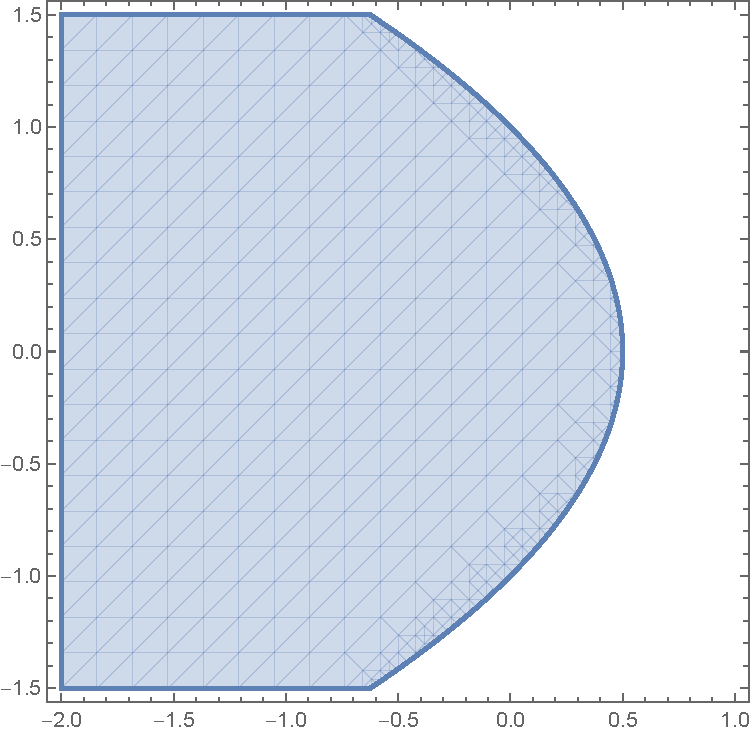
\includegraphics[width=\textwidth]{1.4(1).pdf}
        \caption{(1)}
    \end{minipage}
    \hspace{0.05\textwidth}
    \begin{minipage}[b]{0.45\textwidth}
        \centering
        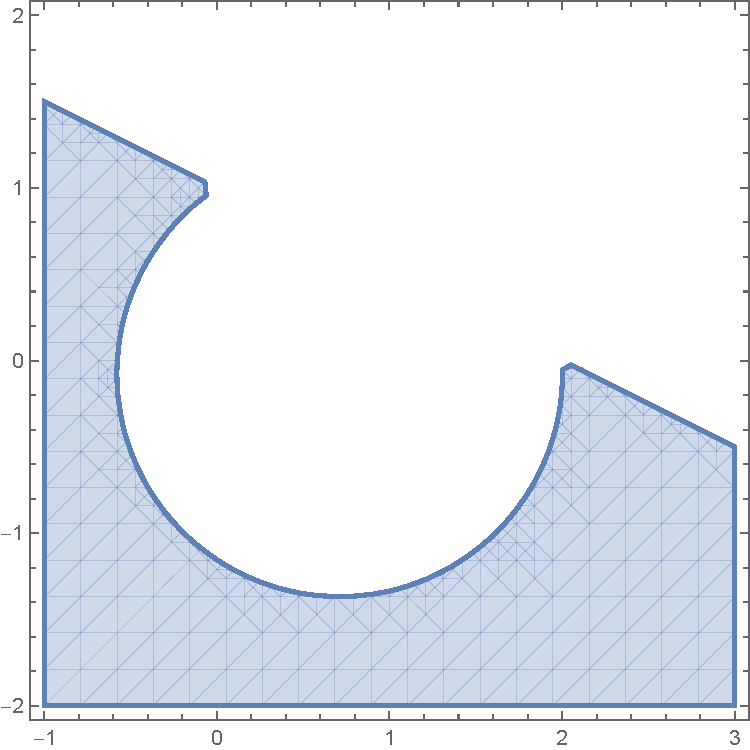
\includegraphics[width=\textwidth]{1.4(2).pdf}
        \caption{(2)}
    \end{minipage}
\end{figure}
\end{sol}\par

\begin{sol}[5]
    $$\begin{aligned}
        &e^{\i n\theta}\\
        =&(\cos\theta+\i\sin\theta)^n\\
        =&\sum_{k=0}^{n}\i^{n-k}C_n^k\cos^k\theta\sin^{n-k}\theta
    \end{aligned}$$
    取实部之后得到
    $$\cos n\theta=\cos^n\theta-C_n^2\cos^{n-2}\theta\sin^2\theta+C_n^4\cos^{n-4}\theta\sin^4\theta+\cdots$$
    取虚部之后得到
    $$\sin n\theta=C_n^1\cos^{n-1}\theta\sin\theta-C_n^3\cos^{n-3}\theta\sin^3\theta+C_n^5\cos^{n-5}\theta\sin^5\theta+\cdots$$
\end{sol}\par

\begin{sol}[6]
    设$z=\sin(\omega)$,则$\omega=\arcsin z$
    $$\begin{aligned}
        z&=\frac{e^{\i\omega}-e^{-\i\omega}}{2\i}\\
        2\i z&=e^{\i\omega}-e^{-\i\omega}\\
        e^{\i2\omega}-2\i ze^{\i\omega}-1&=0\\
        e^{\i\omega}&=\frac{2\i z+\sqrt{-4z^2+4}}{2}\\
        e^{\i\omega}&=\i z+\sqrt{1-z^2}\\
        \omega&=\frac{1}{\i}\ln(\i z+\sqrt{1-z^2})
    \end{aligned}$$
    $\omega$还有另一解$\frac{1}{\i}\ln(\i z-\sqrt{1-z^2})$,但是
    由于$\sqrt{1-z^2}$是多值函数,因此两解等价。    
\end{sol}\par

\begin{sol}[7]
    由三角函数的级数定义知
    $$\begin{aligned}
        \sin\sqrt{z}&=\sqrt{z}-\frac{z\sqrt{z}}{3!}+\cdots\\
        &=\sqrt{z}(1-\frac{z}{3!}+\cdots)
    \end{aligned}$$
    由于等式右边为一不恒为0的单值函数乘以一多值函数,故$\sin\sqrt{z}$为多值函数。\\
    同理$\cos\sqrt{z}$为单值函数,$\frac{\sin\sqrt{z}}{\sqrt{z}}$为单值函数,$\frac{\cos\sqrt{z}}{\sqrt{z}}$为多值函数。
    $$\begin{aligned}
        \sin(\i\ln z)&=\frac{e^{\i\i\ln z}-e^{-\i\i\ln z}}{2\i}\\
        &=\frac{\frac{1}{z}-z}{2\i}
    \end{aligned}$$    
    故$\sin(\i\ln z)$为单值函数。
\end{sol}\par

\begin{sol}[8]
    (1)$$\begin{aligned}
        &\sqrt[3]{(z-a)(z-b)}\\
        =&\sqrt[3]{r_1r_2}e^{\frac{\i (\theta_1+\theta_2)}{3}}
    \end{aligned}$$
    绕$a$转一圈后函数值变为
    $$\begin{aligned}
        &\sqrt[3]{r_1r_2}e^{\frac{\i (\theta_1+\theta_2+2\pi)}{3}}\\
        =&\sqrt[3]{r_1r_2}e^{\frac{\i (\theta_1+\theta_2)}{3}}e^{\i\frac{2\pi}{3}}
    \end{aligned}$$
    故$a$为支点,同理$b$也是支点。\\
    绕无穷远点逆时针绕一圈相当于顺时针绕有穷远所有点一圈,故绕无穷远点一圈后函数值变为
    $$\begin{aligned}
        &\sqrt[3]{r_1r_2}e^{\frac{\i (\theta_1+\theta_2-4\pi)}{3}}\\
        =&\sqrt[3]{r_1r_2}e^{\frac{\i (\theta_1+\theta_2)}{3}}e^{\i(-\frac{4\pi}{3})}
    \end{aligned}$$
    故无穷远点也是支点。\\
    (2)$$\begin{aligned}
        &\ln\frac{z-a}{z-b}\\
        =&\ln\frac{r_1e^{i\theta_1}}{r_2e^{i\theta_2}}\\
        =&\ln\frac{r_1}{r_2}+\i(\theta_1-\theta_2)\\
    \end{aligned}$$
    绕$a$转一圈后函数值变为
    $$\begin{aligned}
        \ln\frac{r_1}{r_2}+\i(\theta_1-\theta_2+2\pi)
    \end{aligned}$$
    故$a$为支点。\\
    绕$b$转一圈后函数值变为
    $$\begin{aligned}
        \ln\frac{r_1}{r_2}+\i(\theta_1-\theta_2-2\pi)
    \end{aligned}$$
    故$b$为支点。\\
    绕无穷远点逆时针绕一圈相当于顺时针绕有穷远所有点一圈,故绕无穷远点一圈后函数值变为
    $$\begin{aligned}
        \ln\frac{r_1}{r_2}+\i(\theta_1-2\pi-\theta_2+2\pi)
    \end{aligned}$$
    故无穷远点不是支点。

\end{sol}\par

\begin{sol}[9]
    记$z-1=r_1e^{\i\theta_1},z+1=r_2e^{\i\theta_2}$。在$z=0$处$\theta_1=\alpha,\theta_2=\beta$\\
    $$\omega(0)=\ln (1)+\i(\alpha+\beta+\pi)$$
    有$\alpha+\beta+\pi=0$\\
    (a)取该割线时可沿逆时针由底下转到$z=3$
    此时$\Delta\theta_1=\pi,\Delta\theta_2=0$故在此时
    $$\omega(3)=\ln 8+\i(\alpha+\pi+\beta+\pi)=3\ln2+\i\pi$$
    (b)取该割线时可沿顺时针由上面转到$z=3$
    此时$\Delta\theta_1=-\pi,\Delta\theta_2=0$故在此时
    $$\omega(3)=\ln 8+\i(\alpha-\pi+\beta+\pi)=3\ln2-\i\pi$$
    (c)取该割线时a,b的路径取法都是可行的,故此割线上岸处
    $$\omega(3)=3\ln2-\i\pi$$
    下岸处
    $$\omega(3)=3\ln2+\i\pi$$


\end{sol}\par
\end{document}